% Lab retreat 2014 presentation
% Author: Nishanth Koganti
% Date: 2014/07/30

\documentclass[10pt,handout]{beamer}
\usetheme{CambridgeUS}

\usepackage{url}
\usepackage{tikz}
\usepackage{xcolor}
\usepackage{caption}
\usepackage{amsmath}
\usepackage{hyperref}
\usepackage{booktabs}
\usepackage{multicol}
\usepackage{multimedia}
\usepackage{array,colortbl}
\usepackage[absolute,overlay]{textpos}
\usetikzlibrary{arrows,shapes,backgrounds,shapes.misc,fit,positioning}
\graphicspath{{./Images/}}

\newenvironment{reference}[2]
{
  \begin{textblock*}{\textwidth}(#1,#2) 
    \footnotesize 
    \it\bgroup
    \color{red!50!black}}
  {\egroup  
  \end{textblock*}
}

\title[Lab Retreat]{Dynamical Modeling of Clothing Articles using GP-LVM}
\author[Nishanth]{Nishanth Koganti\\Mathematical Informatics Laboratory}
\institute[NAIST]{Nara Institute of Science and Technology}
\date{August 6, 2014}

\AtBeginSection[]
{
  \begin{frame}
    \frametitle{Table of Contents}
    \tableofcontents[currentsection]
  \end{frame}
}

%%%%%%%%%%%%%%%%%%%%%%%%%%%%%%%%%%%%%%%%%%%%%%%%%%%%%%%%%%%%%%%%%%%%%%%%%%%%%%%

\begin{document}

\frame{\titlepage}

\begin{frame}
  \frametitle{Contents}
  \tableofcontents
\end{frame}

%%%%%%%%%%%%%%%%%%%%%%%%%%%%%%%%%%%%%%%%%%%%%%%%%%%%%%%%%%%%%%%%%%%%%%%%%%%%%%%

\section{Introduction}

\begin{frame}
\frametitle{Robotic Clothing Assistance}

\begin{itemize}
  \item \textcolor{blue}{Clothing Assistance}: Necessity in the daily life of the elderly and disabled people.\\~\\
  \item Challenging problem involving close interaction of the robot \emph{with non-rigid clothing material and assisted person with varying posture}.  
\end{itemize}

\begin{columns}
  \begin{column}[t]{0.48\textwidth}
    \centering
    \begin{figure}
      \caption*{Non-rigid clothing material}
      \includegraphics[width=0.8\textwidth]{cloth.png}
    \end{figure}
  \end{column}
  \begin{column}[t]{0.48\textwidth}
    \centering
    \begin{figure}
      \caption*{Varying posture of assisted person}
      \includegraphics[width=0.8\textwidth]{posture.png}
    \end{figure}
  \end{column}
\end{columns}

\end{frame}

\begin{frame}
\frametitle{Estimation of Human-Cloth Relationship}

Accurate estimation of human-cloth relationship is crucial to ensure efficient learning of motor skills.\\~\\

We have previously shown that low-cost depth sensor can be used for real-time estimation with key features:

\begin{itemize}
  \item Use of low-dimensional representation for human-cloth relationship (\textcolor{blue}{Topology Coordinates})
  \item Use of compact representation for clothing articles (\textcolor{blue}{Ellipse approximation})
\end{itemize}

\begin{figure}
  \centering
  \includegraphics[width=0.7\textwidth,height=0.5\textheight]{presentsetup.pdf}
\end{figure}

\end{frame}

%%%%%%%%%%%%%%%%%%%%%%%%%%%%%%%%%%%%%%%%%%%%%%%%%%%%%%%%%%%%%%%%%%%%%%%%%%%%%%%

\section{Problem Statement}

\begin{frame}
\frametitle{Problem Statement}

\begin{alertblock}{Problems with previous framework}
Accuracy of human-cloth relationship estimation reduces under:
\begin{itemize}
  \item Occlusion of T-shirt collar from mannequin
  \item Measurement noise in depth sensor
\end{itemize}
\end{alertblock}

~\\~\\

\begin{block}{Proposed Solution}
\textbf{Hypothesis}: Clothing material \textcolor{blue}{follows consistent dynamics} during clothing tasks with minor variations depending on environment\\~\\

\textbf{Proposal}: Extract low-dimensional dynamics model from ground-truth data and use model for \textcolor{blue}{constrained tracking} of human-cloth relationship
\end{block}

\end{frame}

%%%%%%%%%%%%%%%%%%%%%%%%%%%%%%%%%%%%%%%%%%%%%%%%%%%%%%%%%%%%%%%%%%%%%%%%%%%%%%%

\section[GP-LVM]{Gaussian Process Latent Variable Model}

\begin{frame}
\frametitle{What is a Gaussian Process ($\mathcal{GP}$)?}

\emph{Gaussian Process} is a generalization of multivariate gaussian distribution to \textcolor{red}{infinitely many variables}.\\~\\

A Gaussian \textcolor{blue}{distribution} is fully specified by its mean \textcolor{blue}{vector} ($\boldsymbol{\mu}$) and covariance \textcolor{blue}{matrix} ($\boldsymbol{\Sigma}$):

\begin{equation}
  \mathbf{f}(\mathbf{x}) \sim \mathcal{N}(\boldsymbol{\mu},\boldsymbol{\Sigma}),~\mathbf{x} = [x_1~x_2~\cdots~x_N]
\end{equation}

A Gaussian \textcolor{blue}{process} is fully specified by its mean \textcolor{blue}{function} ($m(x)$) and covariance \textcolor{blue}{function} ($k(x,x')$):

\begin{equation}
  f(x) \sim \mathcal{GP}(m(x), k(x,x'))
\end{equation}

\end{frame}

\begin{frame}
\frametitle{How is $\mathcal{GP}$ useful?}

$\mathcal{GP}$ can be used as a prior over \textcolor{blue}{functions} forming \textcolor{blue}{non-parametric model}.

\begin{table}
\centering 
\begin{tabular}{c || c | c} 
 & Mapping & Prior \\ [1ex] 
\hline \hline 
Parametric & $f(\mathbf{X},\theta) = \mathbf{W}\mathbf{X}$ & On function parameters $p(\theta)$ \\ [1ex]
\hline
Non-parametric & $f(x) \sim \mathcal{GP}(m(x),k(x,x'))$ & On function itself $p(f)$\\ [1ex] 
\end{tabular}
\end{table}

\textcolor{blue}{Posterior/Predictive} distribution will also be a $\mathcal{GP}$.

\begin{columns}[t]
  \begin{column}[t]{0.48\textwidth}
    \centering
    \begin{figure}
      \caption*{$\mathcal{GP}$ Regression}
      \includegraphics[width=0.6\textwidth]{gpregression.png}
    \end{figure}
  \end{column}
  \begin{column}[t]{0.48\textwidth}
    \centering
    \begin{figure}
      \caption*{$\mathcal{GP}$ Classification}
      \includegraphics[width=0.6\textwidth]{gpclassification.png}
    \end{figure}
  \end{column}
\end{columns}

\end{frame}

\begin{frame}
\frametitle{Covariance Functions}

\emph{Mean Function} $m(x)$: For most applications using zero mean function is sufficient.\\~\\

\emph{Covariance Function} $k(x,x')$: Defines prior properties of functions sampled from $\mathcal{GP}$ such as: \textcolor{blue}{Stationarity}, \textcolor{blue}{Smoothness}, \textcolor{blue}{Length-scales}.\\~\\

Squared Exponential Covariance Function: 

\begin{equation}
  k(x,x')  = \alpha~\text{exp} \left( - \frac{\gamma}{2} (x - x')^T(x - x') \right),~\alpha,\gamma: \text{hyperparameters}
\end{equation}

\begin{figure}
  \centering
  \includegraphics[width=0.8\textwidth,height=0.4\textheight]{covfunc.jpg}
\end{figure}

\end{frame}

\begin{frame}
\frametitle{Motivation for Dimensionality Reduction}

\begin{itemize}
  \item For data with underlying ``structure'', we expect:
    \begin{itemize}
      \item Fewer distortions than dimensions.
      \item Data to lie on a low-dimensonal manifold.
    \end{itemize}
  \item Conclusion: Deal with high-dimensional data by looking for low-dimensional embedding.
\end{itemize}

\end{frame}

\begin{frame}
\frametitle{Motivation for Dimensionality Reduction}

\begin{center}
  \textbf{UPSC Handwritten Digit Dataset}
\end{center}

\begin{columns}[t]
  \begin{column}[t]{0.3\textwidth}
    \centering
    3648 dimensional space
    \begin{figure}
      \centering
      \caption*{Digit 6 Image}
      
\includegraphics[width=0.3\textwidth]{digitIm1.png}
    \end{figure}
    \begin{figure}
      \centering
      \caption*{Random Image}
      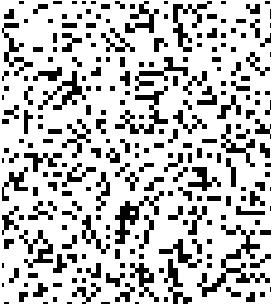
\includegraphics[width=0.3\textwidth]{digitIm2.png}
    \end{figure}
  \end{column}
  \begin{column}{0.6\textwidth}
    \centering
    Low-dimensional manifold for digit rotation
    \begin{figure}
      \centering
      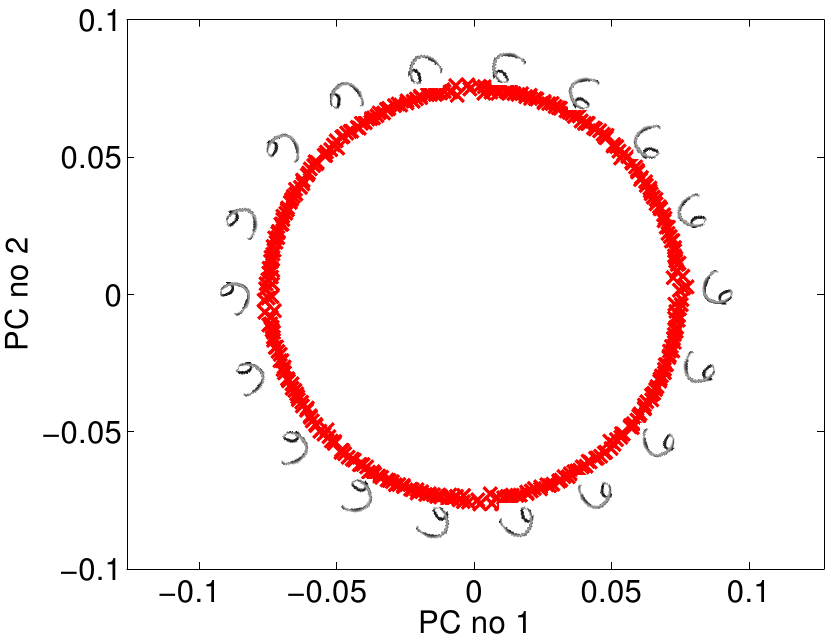
\includegraphics[width=0.8\textwidth]{pca1.png}
    \end{figure}    
  \end{column}
\end{columns}

\end{frame}

\begin{frame}
\frametitle{Probabilistic Generative Model}

\begin{itemize}
  \item \textcolor{blue}{Observed} (high-dimensional) data: $\mathbf{Y} = [y_1~y_2~\cdots~y_N]^T \in \mathbb{R}^{N \times D}$      
  \item \textcolor{blue}{Latent} (low-dimensional) data: $\mathbf{X} = [x_1~x_2~\cdots~x_N]^T \in \mathbb{R}^{N \times Q},~Q << D$
  \item Assume a relationship/mapping of the form:
    \begin{equation}
      \begin{array}{c}
        y_i = \mathbf{W}x_i + \epsilon_i,~\epsilon_i \sim \mathcal{N}(\mathbf{0},\sigma^2\mathbf{I})\\~\\
        y_i = f(x_i) = \epsilon_i
      \end{array}
    \end{equation}
  \item Resultant likelihood on the data:
    \begin{equation}
      p(\mathbf{Y}|\mathbf{X},\mathbf{W}) = \prod_{i = 1}^N \mathcal{N}(y_i | \mathbf{W}x_i, \sigma^2\mathbf{I})
    \end{equation}
\end{itemize}

\end{frame}

\begin{frame}
\frametitle{Probabilistic Generative Model}

\begin{columns}
  \begin{column}[t]{0.48\textwidth}
    \centering
    \textbf{Probabilistic PCA}
    \begin{figure}
      \centering
      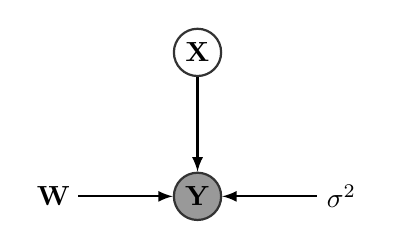
\begin{tikzpicture}
        \tikzstyle{main}=[circle, minimum size = 6mm, thick, draw =black!80, node distance = 12mm]
        \tikzstyle{main1}=[circle, minimum size = 6mm, thick, draw = white, node distance = 12mm]
        \tikzstyle{connect}=[-latex, thick]
        \node[main,fill=black!40] (y) [label=center:$\mathbf{Y}$] {};
        \node[main] (x) [above=of y,label=center:$\mathbf{X}$] {};
        \node[main1] (w) [left=of y,label=center:$\mathbf{W}$] {};
        \node[main1] (sigma) [right=of y,label=center:$\sigma^2$] {};
        \path (x) edge [connect] (y)
        (w) edge [connect] (y)
        (sigma) edge [connect] (y);
      \end{tikzpicture}
    \end{figure}
    Places prior on latent space $\mathbf{X}$ and optimises linear mapping $\mathbf{W}$
    \begin{equation}
      \begin{array}{c}
        p(\mathbf{X}) = \prod_{i=1}^N \mathcal{N}(x_i|\mathbf{0},\mathbf{I})\\~\\
        p(\mathbf{Y}|\mathbf{W},\sigma^2) = \int p(\mathbf{Y}|\mathbf{W},\mathbf{X},\sigma^2)~p(\mathbf{X})
      \end{array}
    \end{equation}
  \end{column}
  \begin{column}[t]{0.48\textwidth}
    \centering
    \textbf{Dual Probabilistic PCA}
    \begin{figure}
      \centering
      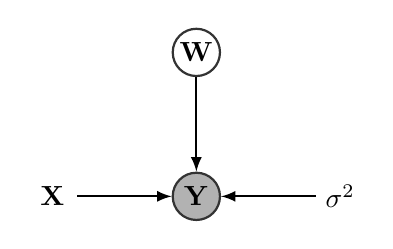
\begin{tikzpicture}
        \tikzstyle{main}=[circle, minimum size = 6mm, thick, draw = black!80, node distance = 12mm]
        \tikzstyle{main1}=[circle, minimum size = 6mm, thick, draw = white, node distance = 12mm]
        \tikzstyle{connect}=[-latex, thick]
        \node[main,fill=black!30] (y) [label=center:$\mathbf{Y}$] {};
        \node[main] (w) [above=of y,label=center:$\mathbf{W}$] {};
        \node[main1] (x) [left=of y,label=center:$\mathbf{X}$] {};
        \node[main1] (sigma) [right=of y,label=center:$\sigma^2$] {};
        \path (x) edge [connect] (y)
        (w) edge [connect] (y)
        (sigma) edge [connect] (y);
      \end{tikzpicture}
    \end{figure}
    Places prior on linear mapping $\mathbf{W}$ and optimises latent space $\mathbf{X}$ 
    \begin{equation}
      \begin{array}{c}
        p(\mathbf{W}) = \prod_{i=1}^D \mathcal{N}(w_i|\mathbf{0},\mathbf{I})\\~\\
        p(\mathbf{Y}|\mathbf{X},\sigma^2) = \int p(\mathbf{Y}|\mathbf{W},\mathbf{X},\sigma^2)~p(\mathbf{W})
      \end{array}
    \end{equation}
  \end{column}
\end{columns}

\end{frame}

\begin{frame}
\frametitle{From Dual PPCA to GP-LVM}

\begin{exampleblock}{}
  \centering
  PPCA and Dual PPCA are equivalent eigenvalue problems with same Maximum Likelihood solution
\end{exampleblock}

\begin{itemize}
  \item \textcolor{blue}{GP-LVM}: Instead of placing prior $p(\mathbf{W})$ on the function parameters in Dual PPCA, we can place a prior $p(f)$ directly on the mapping function i.e. \textcolor{blue}{$\mathcal{GP}$ Prior}\\~\\
  \item A $\mathcal{GP}$ Prior allows for \textcolor{blue}{non-linear mappings} if the covariance function is non-linear. For example, the SE Covariance Function:
    \begin{equation}
      k(x,x') = \alpha~\text{exp} \left( - \frac{\gamma}{2} (x - x')^T(x - x') \right)
    \end{equation}
\end{itemize}

\begin{figure}
  \centering
  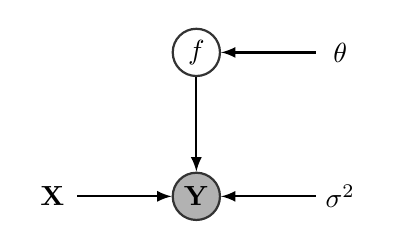
\begin{tikzpicture}
    \tikzstyle{main}=[circle, minimum size = 6mm, thick, draw = black!80, node distance = 12mm]
    \tikzstyle{main1}=[circle, minimum size = 6mm, thick, draw = white, node distance = 12mm]
    \tikzstyle{connect}=[-latex, thick]
    \node[main,fill=black!30] (y) [label=center:$\mathbf{Y}$] {};
    \node[main] (f) [above=of y,label=center:$f$] {};
    \node[main1] (theta) [right=of f,label=center:$\theta$] {};
    \node[main1] (x) [left=of y,label=center:$\mathbf{X}$] {};
    \node[main1] (sigma) [right=of y,label=center:$\sigma^2$] {};
    \path (x) edge [connect] (y)
    (f) edge [connect] (y)
    (sigma) edge [connect] (y)
    (theta) edge [connect] (f);
  \end{tikzpicture}
\end{figure}

\end{frame}

\begin{frame}
\frametitle{Difficulty with Non-linear Mapping}

\begin{itemize}
  \item Normalization of probability distribution after passing through non-linear mapping becomes difficult:
    \begin{figure}
      \centering
      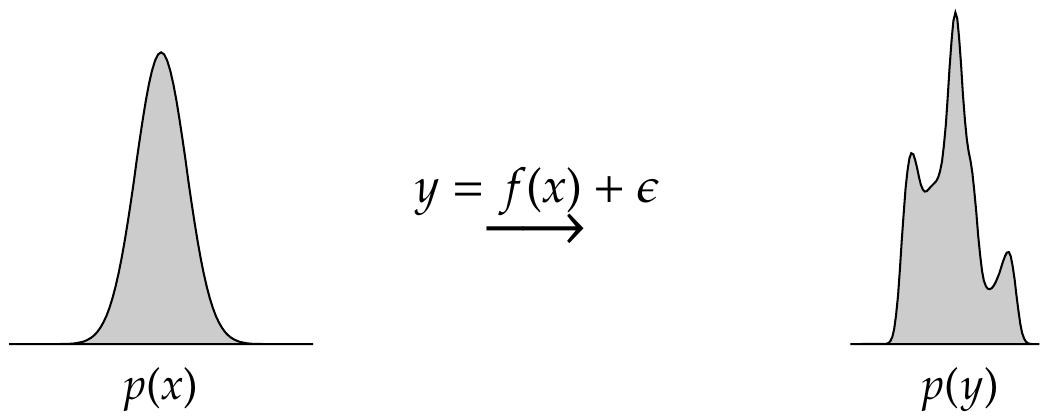
\includegraphics[width=0.5\textwidth]{nonlinear2.png}
    \end{figure}
    
  \item No longer possible to optimize wrt $\mathbf{X}$ as an eigen value problem
    \begin{equation}
      \mathbf{X},\theta = \text{argmax}_{\mathbf{X},\theta} p(\mathbf{Y}|\mathbf{X},\theta)
    \end{equation}

  \item Instead we need to use iterative approach and find gradients wrt $\mathbf{X},\alpha,\gamma,\sigma^2$ 
    
\end{itemize}

\end{frame}

\begin{frame}
\frametitle{Linear vs. Non-linear Dimensionality Reduction}

\begin{figure}
  \centering
  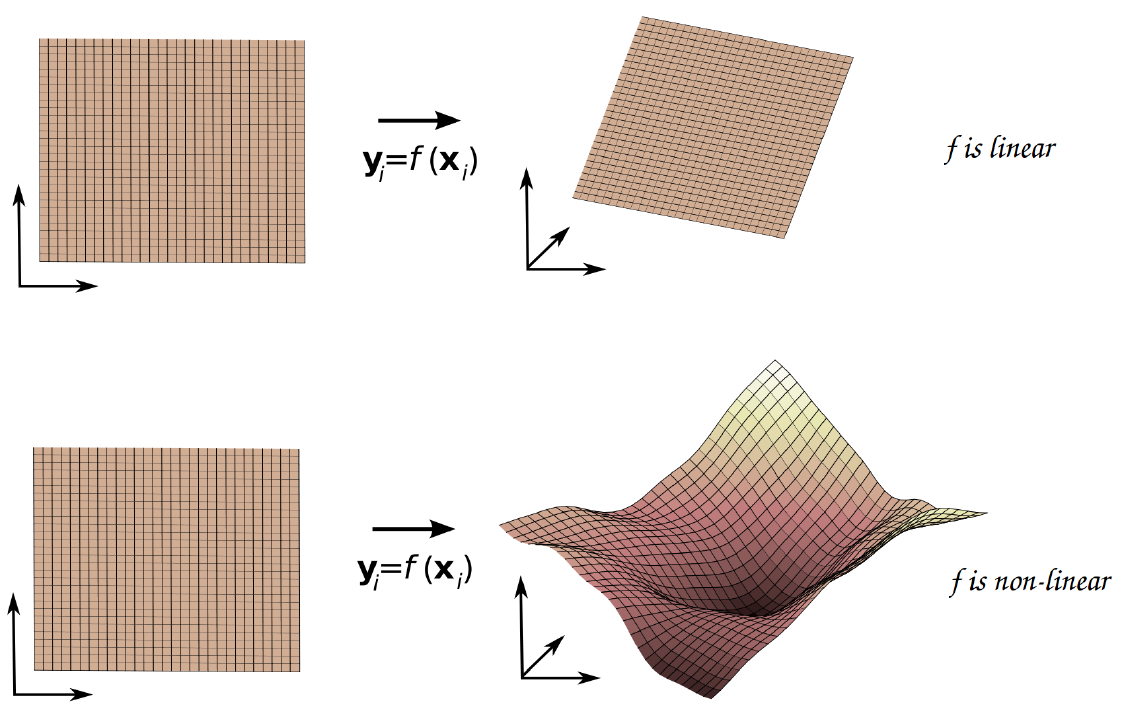
\includegraphics[width=0.8\textwidth]{mapping.png}
\end{figure}

\end{frame}

\begin{frame}
\frametitle{Extensions of GP-LVM}

\textbf{Back Constrained GP-LVM}: Ensures points close in the observation space ($Y$) will be close in latent space by constraining back mapping $f': Y \rightarrow X$\\~\\

\textbf{GP-LVM with Dynamics Model}: Computes latent space assuming that the latent positions ($\mathbf{X}$) are sequential:

\begin{equation}
  x_t = h(x_{t-1}) + \epsilon_{dyn}, \epsilon_{dyn} \sim \mathcal{N}(\mathbf{0},\sigma^2_{dyn}\mathbf{I})
\end{equation}

A $\mathcal{GP}$ Prior is placed on the function $h(x)$. The resultant optimization becomes:

\begin{equation}
  \mathbf{X},\theta,\theta_{dyn} = \text{argmax}_{\mathbf{X},\theta,\theta_{dyn}}~p(\mathbf{Y}|\mathbf{X},\theta)~p(\mathbf{X}|\theta_{dyn})
\end{equation}

\end{frame}

\begin{frame}
\frametitle{Shared GP-LVM}

\begin{itemize}
  \item Objective: Learn a shared latent structure ($\mathbf{X})$ for two observation spaces ($\mathbf{Y},\mathbf{Z})$ of the same phenomenon

    \begin{figure}
      \centering
      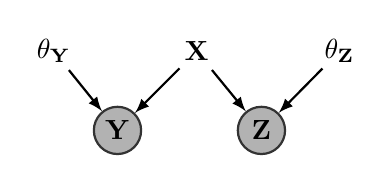
\begin{tikzpicture}
        \tikzstyle{main}=[circle, minimum size = 6mm]
        \tikzstyle{connect}=[-latex, thick]
        \node[main,thick,draw=black!80,node distance=12mm,fill=black!30] (y) [label=center:$\mathbf{Y}$] {};
        \node[main,thick,draw=black!80,node distance=12mm,fill=black!30] (z) [right=of y,label=center:$\mathbf{Z}$] {};
        \node[main,node distance=8mm] (x) [above right=of y,label=center:$\mathbf{X}$] {};
        \node[main,node distance=12mm] (thetay) [left=of x,label=center:$\theta_{\mathbf{Y}}$] {};
        \node[main,node distance=12mm] (thetaz) [right=of x,label=center:$\theta_{\mathbf{Z}}$] {};
        \path (x) edge [connect] (y)
        (x) edge [connect] (z)
        (thetay) edge [connect] (y)
        (thetaz) edge [connect] (z);
      \end{tikzpicture}
    \end{figure}

  \item This model indicates the following:
    \begin{equation}
      \begin{array}{c}
        X,\theta_{\mathbf{Y}},\theta_{\mathbf{Z}} = \text{argmax}_{X,\theta_{\mathbf{Y}},\theta_{\mathbf{Z}}}~p(\mathbf{Y},\mathbf{Z}|X,\theta_{\mathbf{Y}},\theta_{\mathbf{Z}})\\~\\
        = \text{argmax}_{X,\theta_{\mathbf{Y}},\theta_{\mathbf{Z}}}~p(\mathbf{Y}|X,\theta_{\mathbf{Y}})~p(\mathbf{Z}|X,\theta_{\mathbf{Z}})
      \end{array}
    \end{equation}

\end{itemize}

\end{frame}

\begin{frame}
\frametitle{Human Motion Modeling using GP-LVM}

\begin{itemize}
  \item Ek et al. (2007) applied shared GP-LVM to infer human pose from ambiguous silhoutte information.
  \item Extension to Shared GP-LVM:
    \begin{itemize}
      \item Back constraint from pose space ($\mathbf{Z}$)to latent space ($\mathbf{X}$) to enforce \emph{one-to-one} mapping.
      \item Dynamic model in the latent space to enforce representation to follow data's dynamics.
    \end{itemize}
\end{itemize}

\begin{figure}
  \centering
  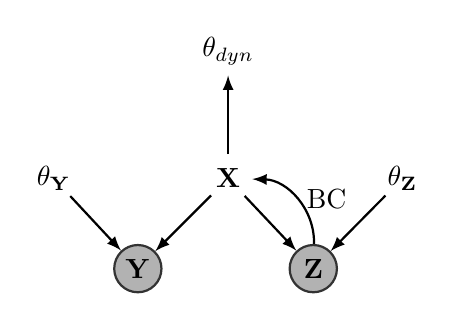
\begin{tikzpicture}
    \tikzstyle{main}=[circle, minimum size = 6mm]
    \tikzstyle{connect}=[-latex, thick]
    \node[main,thick,draw=black!80,node distance=16mm,fill=black!30] (y) [label=center:$\mathbf{Y}$] {};
    \node[main,thick,draw=black!80,node distance=16mm,fill=black!30] (z) [right=of y,label=center:$\mathbf{Z}$] {};
    \node[main,node distance=10mm] (x) [above right=of y,label=center:$\mathbf{X}$] {};
    \node[main,node distance=16mm] (thetay) [left=of x,label=center:$\theta_{\mathbf{Y}}$] {};
    \node[main,node distance=16mm] (thetaz) [right=of x,label=center:$\theta_{\mathbf{Z}}$] {};
    \node[main,node distance=10mm] (thetadyn) [above=of x,label=center:$\theta_{dyn}$] {};
    \path (x) edge [connect] (y)
    (x) edge [connect] (z)
    (z) edge [connect,bend right=45] node[right] {BC} (x)
    (x) edge [connect] (thetadyn)
    (thetay) edge [connect] (y)
    (thetaz) edge [connect] (z);
  \end{tikzpicture}
\end{figure}

\end{frame}

\begin{frame}
\frametitle{Human Pose Inference using Shared GP-LVM}

\begin{figure}
  \centering
  \caption*{Ambiguity in heading direction}
  \includegraphics[width=0.55\textwidth]{humanmodel1.png}
\end{figure}
\begin{figure}
  \centering
  \caption*{Ambiguity in positon of legs}
  \includegraphics[width=0.55\textwidth]{humanmodel2.png}
\end{figure}

\end{frame}
%%%%%%%%%%%%%%%%%%%%%%%%%%%%%%%%%%%%%%%%%%%%%%%%%%%%%%%%%%%%%%%%%%%%%%%%%%%%%%%

\section[Modelling using GP-LVM]{Dynamical Modelling of Clothing Articles}

\begin{frame}
\frametitle{Dynamical Modelling of Clothing Articles}

\centering
\textbf{Objective}: Verify effectiveness of GP-LVM for \textcolor{blue}{clothing assistance task}\\~\\

\begin{columns}
  \begin{column}[c]{0.6\textwidth}
    \centering
    Measured T-shirt collar and sleeve shape using \textcolor{blue}{motion capture system}
    \begin{equation*}
      \begin{array}{c}
        \text{Observed Data, } \mathbf{Y} \in \mathbb{R}^{45}, \text{Location of 15 Markers}\\~\\
        \text{Latent Positions, } \mathbf{X} \in \mathbf{R}^{2}, \text{2-Dimensional space}
      \end{array}
    \end{equation*}
  \end{column}
  \begin{column}[c]{0.4\textwidth}
    \centering
    \begin{figure}
      \includegraphics[width=0.7\textwidth]{markers.png}
    \end{figure}
  \end{column}
\end{columns}

\begin{figure}
  \centering
  \includegraphics[width=0.7\textwidth]{tshirtvar.png}
\end{figure}

\end{frame}

\begin{frame}
\frametitle{Motion Model from Ground-truth Data}

\begin{figure}
  \centering
  \caption*{GP-LVM Model learnt for single clothing trial (N = 141)}
  \includegraphics[width=0.85\textwidth,height=0.8\textheight]{gplvm1.png}
\end{figure}

\end{frame}

\begin{frame}
\frametitle{Motion Model for Multiple Clothing Trials}

\begin{figure}
  \centering
  \caption*{GP-LVM Model learnt for 4 different clothing trials (N = 620)}
  \includegraphics[width=0.85\textwidth,height=0.7\textheight]{gplvm2.png}
\end{figure}

\end{frame}

%%%%%%%%%%%%%%%%%%%%%%%%%%%%%%%%%%%%%%%%%%%%%%%%%%%%%%%%%%%%%%%%%%%%%%%%%%%%%%%

\section[Prediction using Shared GP-LVM]{Cloth State Prediction from Multiple Observations}

\begin{frame}
\frametitle{Cloth State Prediction from Multiple Observations}

\centering
\textbf{Objective}: Infer cloth state from noisy observation and shared GP-LVM model\\~\\

\centering
Measured T-shirt collar and sleeve shape using both \textcolor{blue}{motion capture system} and \textcolor{blue}{kinect depth sensor}

\begin{equation*}
  \begin{array}{c}
    \text{Pose Space, } \mathbf{Z}: \text{Motion Capture Data}\\~\\
    \text{Feature Space, } \mathbf{Y}: \text{Kinect Depth Data}\\~\\
    \text{Latent Space, } \mathbf{X}, \text{5-dimensional representation}
  \end{array}
\end{equation*}

\end{frame}

%\begin{frame}
%\frametitle{Formulation of Shared GP-LVM Model}

%\end{frame}

\begin{frame}
\frametitle{Likelihood over Latent Space}

\begin{figure}
  \centering
  \includegraphics[width=0.8\textwidth,height=0.8\textheight]{likelihood.png}
\end{figure}

\end{frame}

\begin{frame}
\frametitle{State Prediction using Shared GP-LVM}

\centering 
T-shirt state predicted from noisy observation corresponding to latent space point that maximizes likelihood 
\begin{figure}
  \centering
  \includegraphics[width=0.7\textwidth]{prediction.png}
\end{figure}

\end{frame}

\begin{frame}
\frametitle{State Prediction using Shared GP-LVM}

\centering
Euclidean distance error between ground-truth and predicted T-shirt state

\begin{figure}
  \centering
  \includegraphics[width=0.7\textwidth,height=0.7\textheight]{errorModel.pdf}
\end{figure}

\end{frame}

\begin{frame}
\frametitle{Effect of Feature Space Representation}

\centering
Feature space representation plays important role in performance of model

\begin{figure}
  \centering
  \includegraphics[width=0.7\textwidth,height=0.7\textheight]{featureCompare.pdf}
\end{figure}

\end{frame}

%%%%%%%%%%%%%%%%%%%%%%%%%%%%%%%%%%%%%%%%%%%%%%%%%%%%%%%%%%%%%%%%%%%%%%%%%%%%%%%

\section{Conclusion}

\begin{frame}
\frametitle{Conclusion}

\begin{block}{We demonstrated that}
\begin{itemize}
  \item GP-LVM can model dynamics of clothing articles for clothing assistance tasks
  \item Shared GP-LVM can be used to infer true cloth state from noisy depth sensor readings.
\end{itemize}
\end{block}

~\\~\\

\begin{block}{We plan to}
\begin{itemize}
  \item Improve accuracy of Shared GP-LVM by using better representations.
  \item Extend dynamics model to include human posture, robot's proprioceptive information.
\end{itemize}
\end{block}

\end{frame}

\begin{frame}
  \begin{center}
    \Large{Thank you for your kind attention}\\~\\
    \Large{Questions and Comments}
  \end{center}
\end{frame}

%%%%%%%%%%%%%%%%%%%%%%%%%%%%%%%%%%%%%%%%%%%%%%%%%%%%%%%%%%%%%%%%%%%%%%%%%%%%%%%

\section*{Additional Materials}

\end{document}
